\documentclass{standalone}
\usepackage{tikz}

\begin{document}

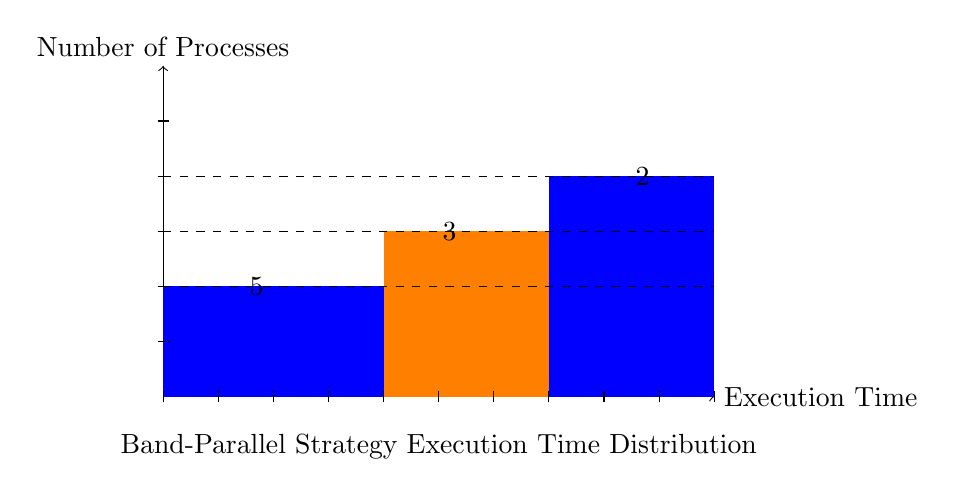
\begin{tikzpicture}[scale=0.7]
    % Set up the axis
    \draw[->] (0,0) -- (10,0) node[right] {Execution Time};
    \draw[->] (0,0) -- (0,6) node[above] {Number of Processes};

    % Draw the bars
    \fill[blue] (0,0) rectangle (4,2); % Between 0 and 40 execution time
    \fill[orange] (4,0) rectangle (7,3); % Between 40 and 80 execution time
    \fill[blue] (7,0) rectangle (10,4); % Between 80 and 100 execution time

    % Add labels
    \node at (2,2) [anchor=east] {5};
    \node at (5.5,3) [anchor=east] {3};
    \node at (9,4) [anchor=east] {2};

    % Add tick marks
    \foreach \x in {0,1,...,10} {
        \draw (\x,-0.1) -- (\x,0.1);
    }
    \foreach \y in {1,2,...,5} {
        \draw (-0.1,\y) -- (0.1,\y);
    }

    % Add grid lines
    \draw[dashed] (0,2) -- (10,2);
    \draw[dashed] (0,3) -- (10,3);
    \draw[dashed] (0,4) -- (10,4);

    % Add title
    \node at (5,-0.5) [below] {Band-Parallel Strategy Execution Time Distribution};
\end{tikzpicture}

\end{document}